\documentclass[12pt, titlepage]{article}
\usepackage[spanish]{babel} 
\usepackage[none]{hyphenat}
\usepackage[margin=3cm]{geometry}
\usepackage{setspace}
\usepackage{parskip}
\usepackage{graphicx}
\usepackage{subcaption}
\usepackage{wrapfig}
\usepackage{fancyhdr}
\usepackage[hidelinks]{hyperref}

\sloppy
\setlength{\parindent}{1.25cm}
\graphicspath{{img/}}
\onehalfspacing
\pagestyle{fancy}
\fancyhead[R]{Acosta Porcayo Alan Omar\\Mecánica}
\setlength{\headheight}{27.69403pt}
\hypersetup{colorlinks=true, urlcolor=blue}
\urlstyle{same}

\begin{document}
    \begin{titlepage}
        \centering
        \begin{figure}[ht]
            \centering
            \begin{subfigure}[r]{0.2\linewidth}
                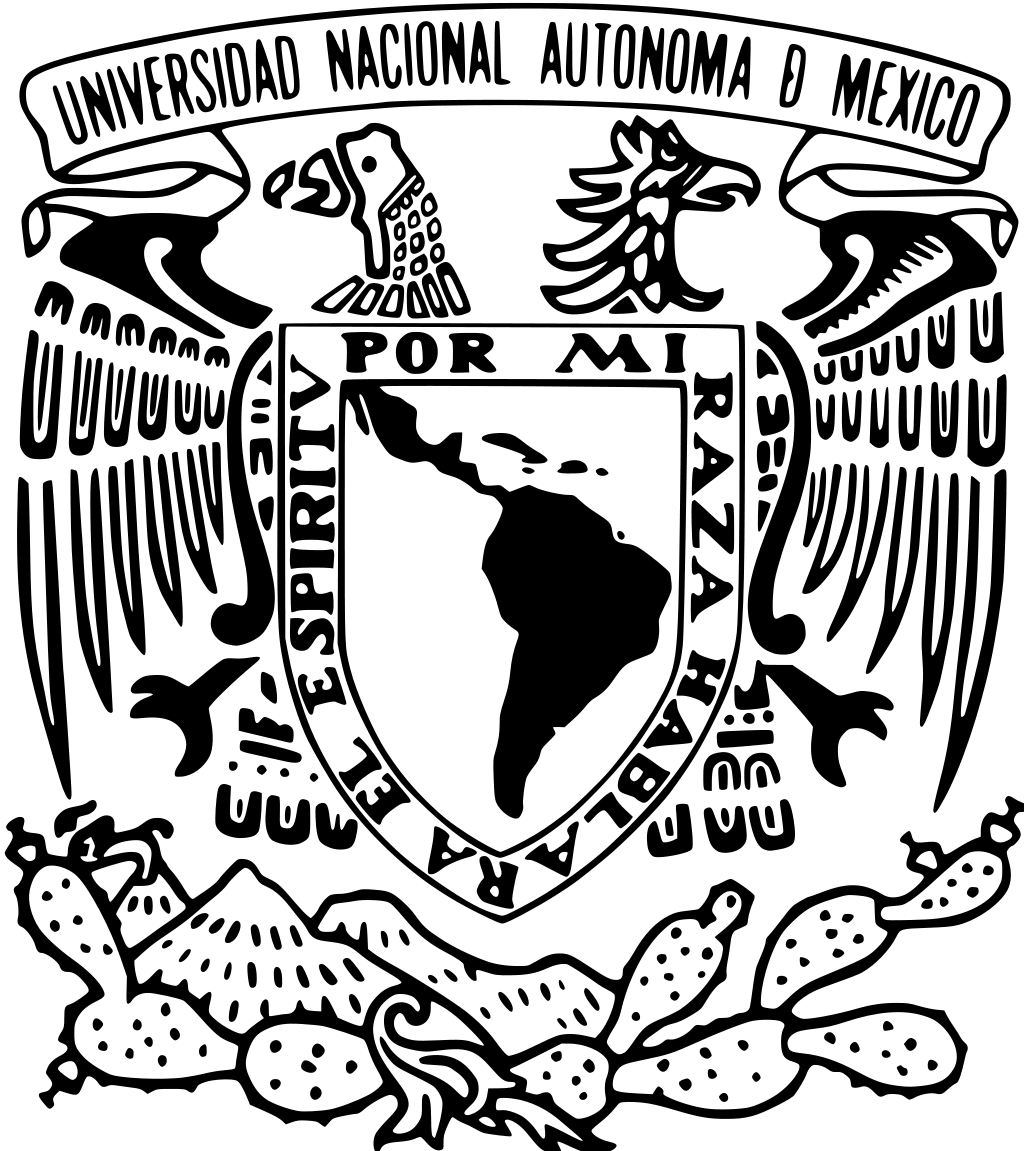
\includegraphics[width=\textwidth]{Escudo_UNAM.png} 
            \end{subfigure} \hspace{9.1cm}
            \begin{subfigure}[l]{0.2\linewidth}
                
\includegraphics[width=\textwidth]{Escudo_FI.png}
            \end{subfigure} 
        \end{figure}

        \large \textbf{UNIVERSDAD NACIONAL AUTÓNOMA DE MÉXICO\\}
        \textbf{\\FACULTAD DE INGENIERÍA\\} 
        \hfill \break
        \Large\textbf{Mecánica\\}
        \textbf{\\La multitarea\\}
        \Large \textbf{\\Nombre del profesor\\}
        \large Lorenzo O. Miranda Cordero\\
        \Large \textbf{\\Grupo 8\\}
        \textbf{\\Alumno:\\}
        Acosta Porcayo Alan Omar\\

        \vspace{1cm}
        \begin{flushright}
            \Large \textbf{Semestre 2023-2}
        \end{flushright}
    \end{titlepage}

    \begin{center}
        \textbf{La multitarea}
    \end{center}
    
    \noindent La multitarea cuanta con algunas interpretaciones, pues mientras algunos la describen como la capacidad para mantener la atención en varias actividades a la vez, otros la explican como ``la eterna disponibilidad'' de una persona. Lo que si está claro es que la multitarea es un fenómeno que se ha normalizado en la época actual y ha tenido un estallido provocado por la era digital.

    En el ámbito tanto educativo como laboral existe la creencia de que la multitarea es una habilidad necesaria para realizar más trabajo, pero lo que en realidad provoca es que las personas comiencen a desgastarse y a rendir menos. 
    
    En mi experiencia he tenido que recurrir a realizar más de una tarea a la vez, ya sea por una gran cantidad de pendientes o por falta de tiempo, y si estoy de acuerdo con la idea de que no es posible prestar atención simultáneamente a todo lo que intento realizar. Por ejemplo, en los trabajos en equipo acostumbro a dialogar con mis compañeros mientras realizamos la actividad, lo que provoca que no se preste la máxima atención a ninguna actividad. 
    
    Otro ejemplo de este problema de distribución de la atención que se menciona en el documental del ``Multitasking'' es el de escuchar música mientras se trabaja o estudia. En mi caso es una práctica que realizo bastante a menudo. Sin embargo, analizando la situación desde esa perspectiva me doy cuenta que es cierto que en ocasiones puedo distraerme por la música de fondo y perder el ritmo de la actividad principal. En otros momentos en los que me centro más en mi actividad principal dejo de escuchar la música y es hasta que tomo un descanso que vuelvo a prestar atención al sonido. 

    Una solución que propone el documental es el de centrarse en una cosa a la vez, de tal manera que se designen tareas especificas y metas concretas para que la persona logre cumplirlas lo mejor posible. También, se deben asignar momentos específicos para taras como responder e-mails o revisar las notificaciones. Este punto me parece que si puede funcionar si se aplica de la manera adecuada, pero puede ser difícil de cambiar en la vida de las personas debido a que la multitarea se ha vuelto algo inconsciente.
    
    Como mencionaba anteriormente, la era digital ha venido a revolucionar la vida de las personas, trayendo sus beneficios pero también sus desventajas. Una de estas desventajas es la ansia de estímulos que sucede principalmente en los adolescentes y adultos jóvenes, provocada por las redes sociales como Instagram, Twitter, TikTok, etc. 

    Esta ansia de estímulos tiene un efecto en el cerebro tal como si fuera una adicción. Los estímulos que provocan sensaciones positivas generan una sustancia llamada dopamina, la cual causa que el individuo busque constantemente más estímulos como interacciones, notificaciones o likes, lo que desarrolla una especie de adicción a estas distracciones.

    Aunque yo no he convertido a las redes sociales en una necesidad para no aburrirme, si reconozco que se ha convertido en un problema muy común. Esto se debe principalmente al tipo de contenido que consume la nueva generación que proviene de aplicaciones como TikTok. La inmediatez del entretenimiento puede provocar una baja retención de la atención, pues la corta duración de los videos provoca que las personas consuman uno tras otro sin tomar conciencia del tiempo que están perdiendo y de la falta de atención a las cosas importantes.  

    En mi caso, no soy una persona que se revise constantemente las redes sociales, principalmente por que no tengo ningún perfil activo, pero si he llegado a experimentar la necesidad de revisar las notificaciones o los correos que interrumpen mis actividades. La época en la que más llegaba a revisar mis dispositivos era durante la pandemia, pues todas las clases eran virtuales y siempre tenia que estar pendiente de cualquier anuncio o tarea nueva. Esta experiencia si llego a generar en mi estrés y tensión debido a que nunca sabia el momento en que me llegaría una notificación y si sería algo bueno o malo.

    A este comportamiento de revisar los dispositivos electrónicos constantemente se le llama la ``disponibilidad digital permanente'', y tal parece que se ha convirtió en un requisito obligatorio que un empleado debe cumplir. Esta practica sin lugar a duda es algo a lo que nos hemos acostumbrado con el tiempo y las soluciones que proponen es crear normas que permitan el derecho a no estar disponible todo el tiempo.

    En este punto estoy completamente de acuerdo, porque si considero un gran problema que sea necesario estar conectado todo el tiempo. En mi experiencia si he pasado periodos largos contestando mensajes y a la vez realizando otras actividades importantes, es por eso que si deberían existir momentos en los que pueda tener la certeza de que no tener interrupciones ni distracciones, de tal manera que elimine esa tensión y me concentre en mis tareas.

    Hasta este momento he mencionado principalmente las desventajas que tiene la multitarea, pero también cabe mencionar las acciones que pueden ayudar a eliminar este problema y cambiar el estilo de vida de las personas. Una técnica de la meditación que mencionan en el documental es la "atención plena", es decir, solo prestar atención al momento presente de manera que se eliminen las preocupaciones por cosas pasadas o futuras. La meditación es algo que nunca he experimentado de primera mano pero parece ser una buena práctica para alcanzar una mejor concentración. 
    
    Una solución más es la de llevar a la realidad las cosas abstractas o complejas, dividiéndolas en partes mas simples y fáciles de comprender, de esta manera se plasman las ideas y perdiendo la menor cantidad de información importante, lo que sería mas difícil si se mantiene esta información en los pensamientos o digitalmente y, aún más, si se tienen distracciones.

    De las formas de plasmar las ideas físicamente, las que acostumbro realizar son las lluvias de ideas y los resúmenes. Los primeras me permiten mencionar los puntos mas importantes que me interesa tocar o resaltar en una actividad, con esto logro evitar olvidar algún punto del que quería expresarme o que considero importante. Los resúmenes principalmente los utilizó para estudiar sobre al algún tema, pues con ellos sintetizo la información mas indispensable y lo estructuro de forma clara para revisar la información en otro momento.
    
    El uso de las redes sociales considero que no han provocado un impacto negativo en mi aprendizaje, esto se debe a que evito utilizarlas en clase y en los momentos en que utilizó mis dispositivos electrónicos son para revisar algún archivo de la clase o para buscar alguna información relativa a mis actividades escolares.

    Finalmente, en el caso de este trabajo lo realice centrándome exclusivamente en exponer mis ideas y reflexiones, evitando distraerme con otras actividades, y percibí que me costó menos esfuerzo del que hubiera necesitado normalmente. Esta actividad me deja como aprendizaje que para realizar mejor un trabajo se debe centrar toda tu atención a tu objetivo y tomarse los descansos adecuados sin cometer el error de distraerse con otras actividades.

    \section*{Bibliografía}
    \noindent DW Documental. (2022, Diciembre 16). Multitasking - ¿Cuánto se puede hacer al mismo tiempo? $|$ DW Documental [Video]. YouTube. \\
    \url{https://www.youtube.com/watch?v=qGQwvd6bd1I}
\end{document}